\documentclass{beamer}

\usepackage[ruled]{algorithm2e}
\SetKw{KwRet}{return}
\SetKwRepeat{Repeat}{repeat}{until}
\usepackage{amsmath}
\usepackage{mathtools}

\usetheme{AnnArbor}
\usecolortheme{crane}
\usefonttheme[onlymath]{serif}

\title{Deep Learning - Foundations and Concepts}
\subtitle{Chapter 15. Discrete Latent Variables}
\author{nonlineark@github}
\date{\today}

\begin{document}

\begin{frame}
    \titlepage
\end{frame}

\begin{frame}
    \frametitle{Outline}
    \tableofcontents
\end{frame}

\section{\texorpdfstring{$K$}{K}-means Clustering}

\begin{frame}
    \frametitle{$K$-means clustering}
    \begin{block}{Problem}
        Suppose we have a data set $\{x^{1},\hdots,x^{N}\}$ consisting of $N$ observations of a $D$-dimensional Euclidean variable $x$. Partition the data set into some number $K$ of clusters, where we will suppose for the moment that the value of $K$ is given.
    \end{block}
\end{frame}

\begin{frame}
    \frametitle{$K$-means clustering}
    \begin{block}{Problem'}
        Find:
        \begin{itemize}
            \item $K$ cluster centers: $\mu_{1},\hdots,\mu_{K}\in\mathbb{R}^{D}$.
            \item $N$ data point assignment: $r^{1},\hdots,r^{N}\in\{\mathrm{e}_{1},\hdots,\mathrm{e}_{K}\}$.
        \end{itemize}
        such that the error function:
        \begin{equation*}
            J=\sum_{n=1}^{N}\sum_{k=1}^{K}r^{n}_{k}||x^{n}-\mu_{k}||^{2}
        \end{equation*}
        which represents the sum of the squares of the distances of each data point to its assigned cluster center, is minimized.
    \end{block}
\end{frame}

\begin{frame}
    \frametitle{$K$-means clustering}
    We can do this through an iterative procedure:
    \begin{enumerate}
        \item Choose some initial values for the $\{\mu_{k}\}$.
        \item E step: Minimize $J$ with respect to the $\{r^{n}_{k}\}$, keeping the $\{\mu_{k}\}$ fixed.
        \item M step: Minimize $J$ with respect to the $\{\mu_{k}\}$, keeping the $\{r^{n}_{k}\}$ fixed.
        \item Go to step 2 until convergence.
    \end{enumerate}
\end{frame}

\begin{frame}
    \frametitle{$K$-means clustering}
    Consider the E step. It's easy to see that we should assign the $n$th data point to the closest cluster center:
    \begin{equation*}
        r^{n}_{k}=\begin{cases}
            1,\qquad\textrm{if }k=\mathrm{argmin}_{j}||x^{n}-\mu_{j}||^{2} \\
            0,\qquad\textrm{otherwise}
        \end{cases}
    \end{equation*}
    For the M step:
    \begin{align*}
        \frac{\partial{}J}{\partial{}\mu_{k}}&=2\sum_{n=1}^{N}r^{n}_{k}(x^{n}-\mu_{k})^{T} \\
        \mu_{k}&=\frac{\sum_{n=1}^{N}r^{n}_{k}x^{n}}{\sum_{n=1}^{N}r^{n}_{k}}
    \end{align*}
    so $\mu_{k}$ is equal to the mean of all the data points $x_{n}$ assigned to cluster $k$.
\end{frame}

\begin{frame}
    \frametitle{$K$-means clustering}
    \begin{algorithm}[H]
        \caption{$K$-means algorithm}
        $\{r^{n}_{k}\}\gets{}0$\;
        \Repeat{$\{r^{n}_{k}\}=\{\prescript{\mathrm{old}}{}{r}^{n}_{k}\}$}{
            $\{\prescript{\mathrm{old}}{}{r}^{n}_{k}\}\gets\{r^{n}_{k}\}$\;
            \For{$n\gets{}1$ \KwTo $N$}{
                $k\gets\mathrm{argmin}_{j}||x^{n}-\mu_{j}||^{2}$\;
                $r^{n}_{k}\gets{}1$\;
                $r^{n}_{j\ne{}k}\gets{}0$\;
            }
            \For{$k\gets{}1$ \KwTo $K$}{
                $\mu_{k}\gets\frac{\sum_{n=1}^{N}r^{n}_{k}x^{n}}{\sum_{n=1}^{N}r^{n}_{k}}$\;
            }
        }
        \Return{$\{\mu_{k}\},\{r^{n}_{k}\}$}\;
    \end{algorithm}
\end{frame}

\begin{frame}
    \frametitle{$K$-means clustering}
    When updating the prototype vectors, we can also derive a sequential update in which, for each data point $x^{n}$ in turn, we update the nearest prototype $\mu_{k}$ using:
    \begin{equation*}
        \prescript{\textrm{new}}{}{\mu}_{k}=\prescript{\textrm{old}}{}{\mu}_{k}+\frac{1}{N_{k}}(x^{n}-\prescript{\textrm{old}}{}{\mu}_{k})
    \end{equation*}
    where $N_{k}$ is the number of data points that have so far been used to update $\mu_{k}$.
\end{frame}

\begin{frame}
    \frametitle{Image segmentation}
    Using the $K$-means algorithm to perform (toy) image segmentation:
    \begin{itemize}
        \item Each pixel in an image is a point in a three-dimensional space comprising the intensities of the red, blue and green channels.
        \item We treat each pixel in the image as a separate data point.
        \item We can apply the $K$-means algorithm to these pixels, and redraw the image in which we replace each pixel by the center $\mu_{k}$ to which that pixel has been assigned.
    \end{itemize}
\end{frame}

\begin{frame}
    \frametitle{Image segmentation}
    \begin{figure}
        \caption{Application of the $K$-means clustering algorithm to image segmentation}
        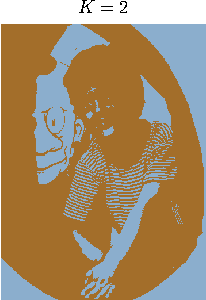
\includegraphics[width=0.2\textwidth]{Figure_3_a.pdf}
        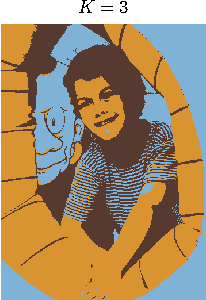
\includegraphics[width=0.2\textwidth]{Figure_3_b.pdf}
        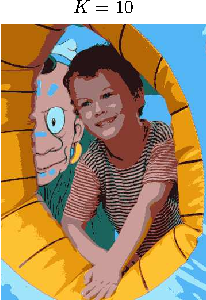
\includegraphics[width=0.2\textwidth]{Figure_3_c.pdf}
        
\includegraphics[width=0.2\textwidth]{Figure_3_d.pdf}
    \end{figure}
\end{frame}

\begin{frame}
    \frametitle{Image segmentation}
    Using the $K$-means algorithm to perform lossy data compression:
    \begin{itemize}
        \item For each of the $N$ data points, we store only the identity $k$ of the cluster to which it is assigned.
        \item We also store the values of the $K$ cluster centers $\{\mu_{k}\}$.
    \end{itemize}
    This framework is often called vector quantization, and the vectors $\{\mu_{k}\}$ are called codebook vectors.
\end{frame}

\section{Mixtures of Gaussians}

\begin{frame}
    \frametitle{Mixtures of Gaussians}
    Formulation of Gaussian mixtures in terms of discrete latent variables:
    \begin{itemize}
        \item Let $z$ be a $K$-dimensional binary random variable having a $1$-of-$K$ representation:
        \begin{itemize}
            \item $p(z)=\prod_{k=1}^{K}\pi_{k}^{z_{k}}$, where $0\le\pi_{k}\le{}1$ and $\sum_{k=1}^{K}\pi_{k}=1$.
        \end{itemize}
        \item Let $x$ be a random variable whose distribution given a particular value for $z$ is a Gaussian:
        \begin{itemize}
            \item $p(x|z)=\prod_{k=1}^{K}\mathcal{N}(x;\mu_{k},\Sigma_{k})^{z_{k}}$.
        \end{itemize}
    \end{itemize}
\end{frame}

\begin{frame}
    \frametitle{Mixtures of Gaussians}
    We see that the marginal distribution for $x$ is given by:
    \begin{equation*}
        p(x)=\sum_{z}p(z)p(x|z)=\sum_{k=1}^{K}\pi_{k}\mathcal{N}(x;\mu_{k},\Sigma_{k})
    \end{equation*}
    which is a Gaussian mixture. We are now able to work with the joint distribution $p(x,z)$ instead of the marginal distribution $p(x)$, and this will lead to significant simplifications.
\end{frame}

\begin{frame}
    \frametitle{Mixtures of Gaussians}
    Let's calculate $\gamma(z_{k})=p(z_{k}=1|x)$:
    \begin{equation*}
        p(z_{k}=1|x)=\frac{p(z_{k}=1)p(x|z_{k}=1)}{\sum_{k'=1}^{K}p(z_{k'}=1)p(x|z_{k'}=1)}=\frac{\pi_{k}\mathcal{N}(x;\mu_{k},\Sigma_{k})}{\sum_{k'=1}^{K}\pi_{k'}\mathcal{N}(x;\mu_{k'},\Sigma_{k'})}
    \end{equation*}
    We will view $\pi_{k}$ as the prior probability of $z_{k}=1$, and the quantity $\gamma(z_{k})$ as the corresponding posterior probability once we have observed $x$. $\gamma(z_{k})$ can also be viewed as the responsibility that component $k$ takes for explaining the observation $x$.
\end{frame}

\begin{frame}
    \frametitle{Likelihood function}
    Suppose we have a data set of observations $\{x^{1},\hdots,x^{N}\}$, and we wish to model this data using a mixture of Gaussians. The log of the likelihood function is given by:
    \begin{equation*}
        L=\sum_{n=1}^{N}\log(\sum_{k=1}^{K}\pi_{k}\mathcal{N}(x^{n};\mu_{k},\Sigma_{k}))
    \end{equation*}
\end{frame}

\begin{frame}
    \frametitle{Likelihood function}
    We see that:
    \begin{itemize}
        \item Due to the presence of the summation over $k$ that appears inside the logarithm, when maximizing this log likelihood function, we will no longer obtain a closed-form solution.
        \item The maximization of the log likelihood function is not a well-posed problem, because singularities will occur whenever one of the Gaussian components collapses onto a specific data point.
        \item Identifiability issue: For any given (non-degenerate) point in the space of parameter values, there will be a further $K!-1$ additional points all of which give rise to exactly the same distribution.
    \end{itemize}
\end{frame}

\begin{frame}
    \frametitle{Maximum likelihood}
    Let's find the conditions that must be satisfied at a maximum of the log likelihood function:
    \begin{align*}
        0&=\frac{\partial{}L}{\partial\mu_{k}}=\sum_{n=1}^{N}\gamma(z^{n}_{k})(x^{n}-\mu_{k})^{T}\Sigma_{k}^{-1}\implies\mu_{k}=\frac{1}{N_{k}}\sum_{n=1}^{N}\gamma(z^{n}_{k})x^{n} \\
        0&=\frac{\partial{}L}{\partial\Lambda_{k}}(H)=\frac{1}{2}\sum_{n=1}^{N}\gamma(z^{n}_{k})\mathrm{tr}((\Sigma_{k}-(x^{n}-\mu_{k})(x^{n}-\mu_{k})^{T})H) \\
        &\implies\Sigma_{k}=\frac{1}{N_{k}}\sum_{n=1}^{N}\gamma(z^{n}_{k})(x^{n}-\mu_{k})(x^{n}-\mu_{k})^{T} \\
        \lambda&=\frac{\partial{}L}{\partial\pi_{k}}=\frac{N_{k}}{\pi_{k}}\implies\pi_{k}=\frac{N_{k}}{N}
    \end{align*}
    where $N_{k}=\sum_{n=1}^{N}\gamma(z^{n}_{k})$. We can interpret $N_{k}$ as the effective number of points assigned to cluster $k$.
\end{frame}

\begin{frame}
    \frametitle{Maximum likelihood}
    We can maximize the log likelihood function through an iterative procedure:
    \begin{enumerate}
        \item Choose some initial values for the means, covariances and mixing coefficients.
        \item E step: Use the current values for the parameters to evaluate the posterior probabilities.
        \item M step: Use these probabilities to re-estimate the means, covariances and mixing coefficients.
        \item Go to step 2 until convergence.
    \end{enumerate}
\end{frame}

\begin{frame}
    \frametitle{Maximum likelihood}
    \scalebox{0.8}{
        \begin{algorithm}[H]
            \caption{EM algorithm for a Gaussian mixture model}
            \Repeat{convergence}{
                \For{$n\gets{}1$ \KwTo $N$}{
                    \For{$k\gets{}1$ \KwTo $K$}{
                        $\gamma(z^{n}_{k})=\frac{\pi_{k}\mathcal{N}(x^{n};\mu_{k},\Sigma_{k})}{\sum_{k'=1}^{K}\pi_{k'}\mathcal{N}(x^{n};\mu_{k'},\Sigma_{k'})}$\;
                    }
                }
                \For{$k\gets{}1$ \KwTo $K$}{
                    $N_{k}\gets\sum_{n=1}^{N}\gamma(z^{n}_{k})$\;
                    $\mu_{k}\gets\frac{1}{N_{k}}\sum_{n=1}^{N}\gamma(z^{n}_{k})x^{n}$\;
                    $\Sigma_{k}\gets\frac{1}{N_{k}}\sum_{n=1}^{N}\gamma(z^{n}_{k})(x^{n}-\mu_{k})(x^{n}-\mu_{k})^{T}$\;
                    $\pi_{k}\gets\frac{N_{k}}{N}$\;
                }
                $L\gets\sum_{n=1}^{N}\log(\sum_{k=1}^{K}\pi_{k}\mathcal{N}(x^{n};\mu_{k},\Sigma_{k}))$\;
            }
            \Return{$\{\mu_{k}\},\{\Sigma_{k}\},\{\pi_{k}\}$}\;
        \end{algorithm}
    }
\end{frame}

\section{Expectation-Maximization Algorithm}

\begin{frame}
    \frametitle{Expectation-maximization algorithm}
    Let's consider the EM algorithm under the more general situation:
    \begin{itemize}
        \item There are $N$ observed data points: $x^{1},\hdots,x^{N}\in\mathbb{R}^{D}$.
        \item The corresponding discrete latent variables $z^{1},\hdots,z^{N}\in\mathbb{R}^{K}$ use a $1$-of-$K$ representation.
        \item The set of all model parameters is denoted by $\theta$.
    \end{itemize}
\end{frame}

\begin{frame}
    \frametitle{Expectation-maximization algorithm}
    The log likelihood function is given by:
    \begin{equation*}
        L=\sum_{n=1}^{N}\log{}p(x^{n};\theta)=\sum_{n=1}^{N}\log(\sum_{z^{n}}p(x^{n},z^{n};\theta))
    \end{equation*}
    The presence of the summation inside the logarithm results in complicated expressions for the maximum likelihood solution.
\end{frame}

\begin{frame}
    \frametitle{Expectation-maximization algorithm}
    The EM algorithm tries to maximize the log likelihood function through an iterative procedure:
    \begin{enumerate}
        \item Choose some starting value for the parameters $\theta_{0}$.
        \item E step: Calculate the posterior distribution of the latent variables $p(z^{n}|x^{n};\theta^{\textrm{old}})$, so that we can form the expected value of the complete-data log likelihood under this posterior distribution $\mathcal{Q}(\theta,\theta^{\textrm{old}})=\sum_{n=1}^{N}\sum_{z^{n}}p(z^{n}|x^{n};\theta^{\textrm{old}})\log{}p(x^{n},z^{n};\theta)$.
        \item M step: We maximize this expectation and determine the revised parameter estimate $\theta^{\textrm{new}}=\mathrm{argmax}_{\theta}\mathcal{Q}(\theta,\theta^{\textrm{old}})$.
        \item Go to step 2 until convergence.
    \end{enumerate}
\end{frame}

\begin{frame}
    \frametitle{Expectation-maximization algorithm}
    \begin{algorithm}[H]
        \caption{General EM algorithm}
        \Repeat{convergence}{
            $\mathcal{Q}(\theta,\theta^{\mathrm{old}})\gets\sum_{n=1}^{N}\sum_{z^{n}}p(z^{n}|x^{n};\theta^{\textrm{old}})\log{}p(x^{n},z^{n};\theta)$\;
            $\theta^{\textrm{new}}\gets\mathrm{argmax}_{\theta}\mathcal{Q}(\theta,\theta^{\textrm{old}})$\;
            $L\gets\sum_{n=1}^{N}\log{}p(x^{n};\theta^{\mathrm{new}})$\;
            $\theta^{\mathrm{old}}\gets\theta^{\mathrm{new}}$\;
        }
        \Return{$\theta^{\mathrm{new}}$}\;
    \end{algorithm}
\end{frame}

\begin{frame}
    \frametitle{Expectation-maximization algorithm}
    \begin{itemize}
        \item The use of the expectation may seem somewhat arbitrary, we will see the motivation for this choice when we give a deeper treatment of EM in Section 15.4.
        \item In the definition of $\mathcal{Q}(\theta,\theta^{\textrm{old}})$, the logarithm acts directly on the joint distribution $p(x^{n},z^{n};\theta)$, and so the corresponding M step maximization will be tractable.
        \item The EM algorithm has the property that each cycle of EM will increase the incomplete-data log likelihood, as we will see in Section 15.4.
    \end{itemize}
\end{frame}

\begin{frame}
    \frametitle{Gaussian mixtures}
    Application of this latent-variable view of EM to the specific case of a Gaussian mixture model. For the E step:
    \begin{align*}
        &p(z^{n}=\mathrm{e}_{k}|x^{n};\theta^{\textrm{old}})=p(z^{n}_{k}=1|x^{n};\theta^{\textrm{old}}) \\
        &=\frac{p(z^{n}_{k}=1,x^{n};\theta^{\textrm{old}})}{\sum_{k'=1}^{K}p(z^{n}_{k'}=1,x^{n};\theta^{\textrm{old}})}=\frac{\pi_{k}^{\textrm{old}}\mathcal{N}(x^{n};\mu_{k}^{\textrm{old}},\Sigma_{k}^{\textrm{old}})}{\sum_{k'=1}^{K}\pi_{k'}^{\textrm{old}}\mathcal{N}(x^{n};\mu_{k'}^{\textrm{old}},\Sigma_{k'}^{\textrm{old}})}=\gamma(z^{n}_{k}) \\
        &\mathcal{Q}(\theta,\theta^{\textrm{old}})=\sum_{n=1}^{N}\sum_{z^{n}}p(z^{n}|x^{n};\theta^{\textrm{old}})\log{}p(x^{n},z^{n};\theta) \\
        &=\sum_{n=1}^{N}\sum_{k=1}^{K}\gamma(z^{n}_{k})(\log\pi_{k}+\log\mathcal{N}(x^{n};\mu_{k},\Sigma_{k}))
    \end{align*}
\end{frame}

\begin{frame}
    \frametitle{Gaussian mixtures}
    For the M step, we fix $\theta^{\textrm{old}}$ thus $\gamma(z^{n}_{k})$, and maximize $\mathcal{Q}(\theta,\theta^{\textrm{old}})$ with respect to $\theta$:
    \begin{align*}
        N_{k}&=\sum_{n=1}^{N}\gamma(z^{n}_{k}) \\
        0&=\frac{\partial\mathcal{Q}}{\partial\mu_{k}}=\sum_{n=1}^{N}\gamma(z^{n}_{k})(x^{n}-\mu_{k})^{T}\Sigma_{k}^{-1}\implies\mu_{k}=\frac{1}{N_{k}}\sum_{n=1}^{N}\gamma(z^{n}_{k})x^{n} \\
        0&=\frac{\partial\mathcal{Q}}{\partial\Lambda_{k}}(H)=\frac{1}{2}\sum_{n=1}^{N}\gamma(z^{n}_{k})\mathrm{tr}((\Sigma_{k}-(x^{n}-\mu_{k})(x^{n}-\mu_{k})^{T})H) \\
        &\implies\Sigma_{k}=\frac{1}{N_{k}}\sum_{n=1}^{N}\gamma(z^{n}_{k})(x^{n}-\mu_{k})(x^{n}-\mu_{k})^{T} \\
        \lambda&=\frac{\partial\mathcal{Q}}{\partial\pi_{k}}=\frac{N_{k}}{\pi_{k}}\implies\pi_{k}=\frac{N_{k}}{N}
    \end{align*}
\end{frame}

\begin{frame}
    \frametitle{Relation to $K$-means}
    We can derive the $K$-means algorithm as a particular limit of EM for Gaussian mixtures. Consider a Gaussian mixture model in which:
    \begin{itemize}
        \item The mixing coefficients are fixed to $\frac{1}{K}$.
        \item The covariance matrices of the mixture components are given by $\epsilon{}I$, where $\epsilon$ is a fixed constant.
    \end{itemize}
\end{frame}

\begin{frame}
    \frametitle{Relation to $K$-means}
    Consider the limit $\epsilon\to{}0+$. For the E step:
    \begin{align*}
        \gamma(z^{n}_{k})&=\frac{\exp(-\frac{||x^{n}-\mu_{k}^{\textrm{old}}||^{2}}{2\epsilon})}{\sum_{k'=1}^{K}\exp(-\frac{||x^{n}-\mu_{k'}^{\textrm{old}}||^{2}}{2\epsilon})} \\
        &\to\begin{cases}
            1,\qquad\textrm{if }k=\mathrm{argmin}_{j}||x^{n}-\mu_{j}^{\textrm{old}}||^{2} \\
            0,\qquad\textrm{otherwise}
        \end{cases}
    \end{align*}
    Thus, in this limit, we obtain a hard assignment of data points to clusters, just as in the $K$-means algorithm, so that $\gamma(z^{n}_{k})\to{}r^{n}_{k}$.
\end{frame}

\begin{frame}
    \frametitle{Relation to $K$-means}
    The expected complete-data log likelihood becomes:
    \begin{align*}
        \epsilon\mathcal{Q}(\theta,\theta^{\textrm{old}})&=\epsilon\sum_{n=1}^{N}\sum_{k=1}^{K}\gamma(z^{n}_{k})(-\log{K}+\log\mathcal{N}(x^{n};\mu_{k},\epsilon{}I)) \\
        &\to-\frac{1}{2}\sum_{n=1}^{N}\sum_{k=1}^{K}r^{n}_{k}||x^{n}-\mu_{k}||^{2}
    \end{align*}
    We see that in this limit, maximizing the expected complete-data log likelihood is equivalent to minimizing the error measure $J$ for the $K$-means algorithm.
\end{frame}

\begin{frame}
    \frametitle{Relation to $K$-means}
    For the M step:
    \begin{equation*}
        \mu_{k}=\frac{\sum_{n=1}^{N}\gamma(z^{n}_{k})x^{n}}{\sum_{n=1}^{N}\gamma(z^{n}_{k})}\to\frac{\sum_{n=1}^{N}r^{n}_{k}x^{n}}{\sum_{n=1}^{N}r^{n}_{k}}
    \end{equation*}
    The EM re-estimation equation for the $\mu_{k}$ then reduces to the $K$-means result.
\end{frame}

\begin{frame}
    \frametitle{Mixtures of Bernoulli distributions}
    As a further example of mixture modelling and to illustrate the EM algorithm in a different context, we now discuss mixtures of descrete binary variables described by Bernoulli distributions:
    \begin{itemize}
        \item Let $z$ be a $K$-dimensional binary random variable having a $1$-of-$K$ respresentation:
        \begin{itemize}
            \item $p(z)=\prod_{k=1}^{K}\pi_{k}^{z_{k}}$, where $0\le\pi_{k}\le{}1$ and $\sum_{k=1}^{K}\pi_{k}=1$.
        \end{itemize}
        \item Let $x\in\mathbb{R}^{D}$ be a set of $D$ binary variables, each of which is governed by a Bernoulli distribution given a particular value for $z$:
        \begin{itemize}
            \item $\mathrm{Bern}(x;\mu)=\prod_{d=1}^{D}\mu_{d}^{x_d}(1-\mu_{d})^{1-x_{d}}$.
            \item $p(x|z)=\prod_{k=1}^{K}\mathrm{Bern}(x;\mu^{k})^{z_{k}}$.
        \end{itemize}
    \end{itemize}
\end{frame}

\begin{frame}
    \frametitle{Mixtures of Bernoulli distributions}
    Application of the EM algorithm to the specific case of a Bernoulli mixture model. For the E step:
    \begin{align*}
        &\gamma(z^{n}_{k})=p(z^{n}=\mathrm{e}_{k}|x^{n};\theta^{\textrm{old}})=p(z^{n}_{k}=1|x^{n};\theta^{\textrm{old}}) \\
        &=\frac{p(z^{n}_{k}=1,x^{n};\theta^{\textrm{old}})}{\sum_{k'=1}^{K}p(z^{n}_{k'}=1,x^{n};\theta^{\textrm{old}})}=\frac{\pi_{k}^{\textrm{old}}\mathrm{Bern}(x^{n};(\mu^{k})^{\textrm{old}})}{\sum_{k'=1}^{K}\pi_{k'}^{\textrm{old}}\mathrm{Bern}(x^{n};(\mu^{k'})^{\textrm{old}})} \\
        &\mathcal{Q}(\theta,\theta^{\textrm{old}})=\sum_{n=1}^{N}\sum_{z^{n}}p(z^{n}|x^{n};\theta^{\textrm{old}})\log{}p(x^{n},z^{n};\theta) \\
        &=\sum_{n=1}^{N}\sum_{k=1}^{K}\gamma(z^{n}_{k})(\log\pi_{k}+\log\mathrm{Bern}(x^{n};\mu^{k}))
    \end{align*}
\end{frame}

\begin{frame}
    \frametitle{Mixtures of Bernoulli distributions}
    For the M step, we fix $\theta^{\textrm{old}}$ thus $\gamma(z^{n}_{k})$, and maximize $\mathcal{Q}(\theta,\theta^{\textrm{old}})$ with respect to $\theta$:
    \begin{align*}
        N_{k}&=\sum_{n=1}^{N}\gamma(z^{n}_{k}) \\
        0&=\frac{\partial\mathcal{Q}}{\partial\mu^{k}_{d}}=\frac{1}{\mu^{k}_{d}(1-\mu^{k}_{d})}\sum_{n=1}^{N}\gamma(z^{n}_{k})(x^{n}_{d}-\mu^{k}_{d}) \\
        &\implies\mu^{k}_{d}=\frac{1}{N_{k}}\sum_{n=1}^{N}\gamma(z^{n}_{k})x^{n}_{d}\implies\mu^{k}=\frac{1}{N_{k}}\sum_{n=1}^{N}\gamma(z^{n}_{k})x^{n} \\
        \lambda&=\frac{\partial\mathcal{Q}}{\partial\pi_{k}}=\frac{N_{k}}{\pi_{k}}\implies\pi_{k}=\frac{N_{k}}{N}
    \end{align*}
\end{frame}

\section{Evidence Lower Bound}

\begin{frame}
    \frametitle{Evidence lower bound}
    We now present an even more general perspective on the EM algorithm by deriving a lower bound on the log likelihood function, which is known as the evidence lower bound or ELBO. Again, the assumptions are:
    \begin{itemize}
        \item There is a probabilistic model in which we denote all the observed variables by $X$ and all the hidden variables by $Z$.  The model is governed by a set of parameters denoted by $\theta$.
        \item Direct optimization of $p(X;\theta)$ is difficult.
        \item Optimization of the complete-data likelihood function $p(X,Z;\theta)$ is significantly easier.
    \end{itemize}
\end{frame}

\begin{frame}
    \frametitle{Evidence lower bound}
    For any distribution $q(Z)$ defined over the latent variables, we have:
    \begin{align*}
        \log{}p(X;\theta)&=\sum_{Z}q(Z)\log{}p(X;\theta) \\
        &=\sum_{Z}q(Z)\log\frac{p(X,Z;\theta)}{p(Z|X;\theta)} \\
        &=\sum_{Z}q(Z)\log\frac{\frac{p(X,Z;\theta)}{q(Z)}}{\frac{p(Z|X;\theta)}{q(Z)}} \\
        &=\sum_{Z}q(Z)\log\frac{p(X,Z;\theta)}{q(Z)}-\sum_{Z}q(Z)\log\frac{p(Z|X;\theta)}{q(Z)} \\
        &=\mathcal{L}(q,\theta)+\mathrm{KL}(q(Z)||p(Z|X;\theta))
    \end{align*}
\end{frame}

\begin{frame}
    \frametitle{Evidence lower bound}
    We see that $\mathrm{KL}(q(Z)||p(Z|X;\theta))$ is the Kullback-Leibler divergence between $q(Z)$ and the posterior distribution $p(Z|X;\theta)$, thus $\mathrm{KL}(q(Z)||p(Z|X;\theta))\ge{}0$, with equality if and only if $q(Z)=p(Z|X;\theta)$. It also follows that:
    \begin{equation*}
        \log{}p(X;\theta)\ge\mathcal{L}(q,\theta)
    \end{equation*}
    In other words that $\mathcal{L}(q,\theta)$ is a lower bound on $\log{}p(X;\theta)$.
\end{frame}

\begin{frame}
    \frametitle{EM revisited}
    In the E step, the lower bound $\mathcal{L}(q,\theta^{\textrm{old}})$ is maximized with respect to $q(Z)$ while holding $\theta^{\textrm{old}}$ fixed. It's easy to see that the solution to this maximization problem is $q(Z)=p(Z|X;\theta)$.
    \begin{figure}
        \caption{Illustration of the E step of the EM algorithm}
        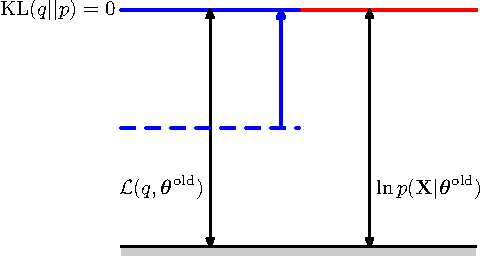
\includegraphics{Figure_14.pdf}
    \end{figure}
\end{frame}

\begin{frame}
    \frametitle{EM revisited}
    In the M step, the distribution $q(Z)$ is held fixed and the lower bound $\mathcal{L}(q,\theta)$ is maximized with respect to $\theta$ to give some new value $\theta^{\textrm{new}}$:
    \begin{itemize}
        \item This will cause the lower bound $\mathcal{L}$ to increase, which will necessarily cause the corresponding log likelihood function to increase.
        \item Because $q(Z)=p(Z|X;\theta^{\textrm{old}})$, it will not equal the new posterior distribution $p(Z|X;\theta^{\textrm{new}})$, and hence there will be a non-zero Kullback-Leibler divergence.
    \end{itemize}
\end{frame}

\begin{frame}
    \frametitle{EM revisited}
    \begin{figure}
        \caption{Illustration of the M step of the EM algorithm}
        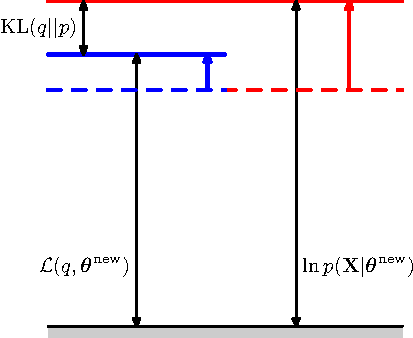
\includegraphics{Figure_15.pdf}
    \end{figure}
\end{frame}

\begin{frame}
    \frametitle{EM revisited}
    Let's take a closer look at the function we try to maximize in the M step:
    \begin{align*}
        &\mathcal{L}(q,\theta)=\sum_{Z}p(Z|X;\theta^{\textrm{old}})\log\frac{p(X,Z;\theta)}{p(Z|X;\theta^{\textrm{old}})} \\
        &=\sum_{Z}p(Z|X;\theta^{\textrm{old}})\log{}p(X,Z;\theta)-\sum_{Z}p(Z|X;\theta^{\textrm{old}})\log{}p(Z|X;\theta^{\textrm{old}}) \\
        &=\mathcal{Q}(\theta,\theta^{\textrm{old}})+\textrm{const}
    \end{align*}
\end{frame}

\begin{frame}
    \frametitle{EM revisited}
    We see that:
    \begin{itemize}
        \item Here we recognize $\mathcal{Q}(\theta,\theta^{\textrm{old}})$ as the expected complete-data log likelihood, and it is therefore the quantity that is being maximized in the M step.
        \item The variable $\theta$ over which we are optimizing appears only inside the logarithm, and by our assumption, the complete-data likelihood function $p(X,Z;\theta)$ is significantly easier to optimize.
    \end{itemize}
\end{frame}

\begin{frame}
    \frametitle{EM revisited}
    \begin{figure}
        \caption{The operation of the EM algorithm viewed in the space of parameters}
        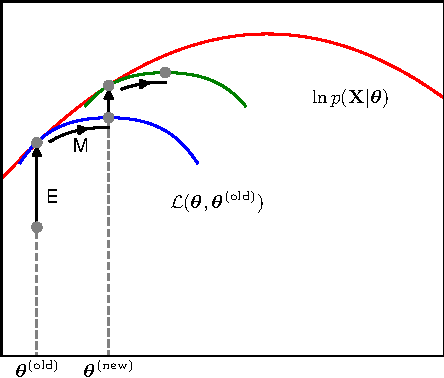
\includegraphics[height=0.7\textheight]{Figure_16.pdf}
    \end{figure}
\end{frame}

\begin{frame}
    \frametitle{EM revisited}
    After each E step, the lower bound curve $\mathcal{L}(q,\theta)$ becomes tangent to the log likelihood curve $\log{}p(X;\theta)$ at $\theta^{\textrm{old}}$:
    \begin{align*}
        \frac{\partial}{\partial\theta}\bigg|_{\theta=\theta^{\textrm{old}}}\mathcal{L}(q,\theta)&=\sum_{Z}\frac{\partial}{\partial\theta}\bigg|_{\theta=\theta^{\textrm{old}}}p(Z|X;\theta^{\textrm{old}})\log\frac{p(X,Z;\theta)}{p(Z|X;\theta^{\textrm{old}})} \\
        &=\frac{1}{p(X;\theta^{\textrm{old}})}\sum_{Z}\frac{\partial}{\partial\theta}\bigg|_{\theta=\theta^{\textrm{old}}}p(X,Z;\theta) \\
        &=\frac{1}{p(X;\theta^{\textrm{old}})}\frac{\partial}{\partial\theta}\bigg|_{\theta=\theta^{\textrm{old}}}\sum_{Z}p(X,Z;\theta) \\
        &=\frac{1}{p(X;\theta^{\textrm{old}})}\frac{\partial}{\partial\theta}\bigg|_{\theta=\theta^{\textrm{old}}}p(X;\theta) \\
        &=\frac{\partial}{\partial\theta}\bigg|_{\theta=\theta^{\textrm{old}}}\log{}p(X;\theta)
    \end{align*}
\end{frame}

\begin{frame}
    \frametitle{Independent and identically distributed data}
    For the particular case of an i.i.d. data set, we have $p(X,Z;\theta)=\prod_{n=1}^{N}p(x^{n},z^{n};\theta)$. Further, we have:
    \begin{align*}
        p(X;\theta)&=\sum_{Z}p(X,Z;\theta) \\
        &=\sum_{z^{1}}\cdots\sum_{z^{N}}p(x^{1},z^{1};\theta)\cdots{}p(x^{N},z^{N};\theta) \\
        &=\sum_{z^{1}}p(x^{1},z^{1};\theta)\cdots\sum_{z^{N}}p(x^{N},z^{N};\theta) \\
        &=p(x^{1};\theta)\cdots{}p(x^{N};\theta) \\
        p(Z|X;\theta)&=\frac{p(X,Z;\theta)}{p(X;\theta)}=\frac{\prod_{n=1}^{N}p(x^{n},z^{n};\theta)}{\prod_{n=1}^{N}p(x^{n};\theta)}=\prod_{n=1}^{N}p(z^{n}|x^{n};\theta)
    \end{align*}
\end{frame}

\begin{frame}
    \frametitle{Independent and identically distributed data}
    \begin{align*}
        \mathcal{Q}(\theta,\theta^{\textrm{old}})&=\sum_{Z}p(Z|X;\theta^{\textrm{old}})\log{}p(X,Z;\theta) \\
        &=\sum_{z^{1}}\cdots\sum_{z^{N}}p(z^{1}|x^{1};\theta^{\textrm{old}})\cdots{}p(z^{N}|x^{N};\theta^{\textrm{old}})\sum_{n=1}^{N}\log{}p(x^{n},z^{n};\theta) \\
        &=\sum_{n=1}^{N}\sum_{z^{1}}\cdots\sum_{z^{N}}p(z^{1}|x^{1};\theta^{\textrm{old}})\cdots{}p(z^{N}|x^{N};\theta^{\textrm{old}})\log{}p(x^{n},z^{n};\theta) \\
        &=\sum_{n=1}^{N}\sum_{z^{n}}p(z^{n}|x^{n};\theta^{\textrm{old}})\log{}p(x^{n},z^{n};\theta)
    \end{align*}
    This is exactly the form that was given when we formally introduced the EM algorithm in Section 15.3. We see that the form given here is more general. 
\end{frame}

\begin{frame}
    \frametitle{Parameter priors}
    We can also use the EM algorithm to maximize the postierior distribution $p(\theta|X)$ for models in which we have introduced a prior $p(\theta)$ over the parameters:
    \begin{align*}
        \log{}p(\theta|X)&=\log{}p(X,\theta)-\log{}p(X) \\
        &=\log{}p(X|\theta)+\log{}p(\theta)-\log{}p(X) \\
        &=\mathcal{L}(q,\theta)+\mathrm{KL}(q(Z)||p(Z|X,\theta))+\log{}p(\theta)-\log{}p(X) \\
        &\ge\mathcal{L}(q,\theta)+\log{}p(\theta)-\log{}p(X)
    \end{align*}
    The E step is the same as the standard EM algorithm, while the M-step equations are modified through the introduction of the prior term $\log{}p(\theta)$.
\end{frame}

\begin{frame}
    \frametitle{Generalized EM}
    For complex models it may be the case that either the E step or the M step, or indeed both, remain intractable:
    \begin{itemize}
        \item The generalized EM algorithm addresses the problem of an intractable M step:
        \begin{itemize}
            \item One way would be to use gradient-based iterative optimization algorithm during the M step.
            \item The expectation conditional maximization algorithm involves making several constrained optimizations within each M step.
        \end{itemize}
        \item We can similarly generalize the E step of the EM algorithm by performing a partial, rather than complete, optimization of $\mathcal{L}(q,\theta)$ with respect to $q(Z)$.
    \end{itemize}
\end{frame}

\begin{frame}
    \frametitle{Sequential EM}
    Incremental form of EM:
    \begin{itemize}
        \item In the E step, we just re-evaluate the responsibilities for one data point.
        \item In the M step, update the required sufficient statistics incrementally.
    \end{itemize}
\end{frame}

\begin{frame}
    \frametitle{Sequential EM}
    For intance, for a Gaussian mixture, suppose we perform an update for data point $m$:
    \begin{align*}
        \gamma^{\textrm{new}}(z^{m}_{k})&=\cdots \\
        N^{\textrm{new}}_{k}&=N^{\textrm{old}}_{k}-\gamma^{\textrm{old}}(z^{m}_{k})+\gamma^{\textrm{new}}(z^{m}_{k}) \\
        \mu^{\textrm{new}}_{k}&=\mu^{\textrm{old}}_{k}+\frac{\gamma^{\textrm{new}}(z^{m}_{k})-\gamma^{\textrm{old}}(z^{m}_{k})}{N^{\textrm{new}}_{k}}(x^{m}-\mu^{\textrm{old}}_{k})
    \end{align*}
    The corresponding results for the covariances and the mixing coefficients are analogous.
\end{frame}

\end{document}